% =========================================================================== %

\begin{frame}[t,plain]
\titlepage
\end{frame}

% =========================================================================== %

\begin{frame}{Recap: Exceptions}
%
\begin{columns}[T]
\column{.5\linewidth}
\begin{itemize}
\item Block structure
	\begin{itemize}
	\item \inPy{try}: Anything that might go wroing
	\item \inPy{except}: What to do if something goes wrong
	\item \inPy{else}: What to do if everything is all right
	\item \inPy{finally}: What to do in any case
	\end{itemize}
\item Error Classes
	\begin{itemize}
	\item Hierarchical Order
	\item Allows specific treatment
	\end{itemize}
\end{itemize}
%
\column{.5\linewidth}
\begin{itemize}
\item Command \inPy{raise}
	\begin{itemize}
	\item Trigger an exception yourself
	\item Argument: instance of an error class
	\item Or: Re-raise in an \inPy{except} block
	\end{itemize}
\item Own Error Classes
	\begin{itemize}
	\item Inherit from \inPy{class} \inPy{Exception}
	\item Arbitrary Design
	\item Usually only for specific treatment of user-defined errors: \enquote{empty} classes
	\end{itemize}
\end{itemize}
\end{columns}
%
\begin{center}
	\emph{Any Questions?}
\end{center}
%
\end{frame}

% =========================================================================== %

\begin{frame}[fragile]{Chapter 10}
%
\begin{itemize}
\item Basics of the MatPlotLib
\item Manipulating Plot Details
\item Different Plot Types
\end{itemize}
%
\end{frame}

% =========================================================================== %

\begin{frame}[fragile]{A First Example}
%
\begin{codebox}[Example: A Simple Plot, width=.53\linewidth, nobeforeafter, equal height group = grpXmpSimplePlot]
\begin{minted}[linenos, fontsize=\scriptsize]{python3}
import math
import matplotlib.pyplot as plt

N = 100
X = [(x - N/2) / 10 for x in range(N)]
Y = [math.sin(x) for x in X]

plt.plot(X, Y)
plt.show()
\end{minted}
\end{codebox}
%
\begin{tcolorbox}[title=Output: A Simple Plot, width=.45\linewidth, nobeforeafter, equal height group = grpXmpSimplePlot]
	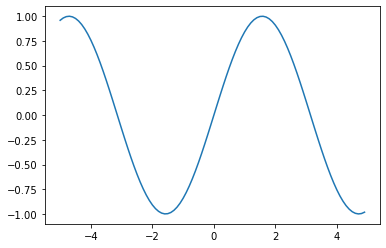
\includegraphics[width=\linewidth]{./gfx/plt-sin}
\end{tcolorbox}
%
\end{frame}

% =========================================================================== %

\begin{frame}[fragile]{Code Analysis}
%
%\small
\begin{itemize}
\item \inPy{import matplotlib.pyplot as plt}
	\begin{itemize}
	\item Module \texttt{matplotlib.pyplot} brings tons of functions
	\item Highly complex structure -- organized into sub-modules
	\item Convention: load as \texttt{plt} to spare us typing this over and over
	\end{itemize}
\item Objects \texttt{X, Y}
	\begin{itemize}
	\item Data to plot: Coordinates
	\item Simple lists of numbers, same length
	\end{itemize}
\item \inPy{plt.plot(X, Y)}
	\begin{itemize}
	\item Prepare the plot in memory
	\item Allows for alterations to the default settings
	\end{itemize}
\item \inPy{plt.show()}
	\begin{itemize}
	\item \enquote{Go live}
	\item Show the plot on screen
	\item Wait with execution until plot window is closed
	\end{itemize}
\end{itemize}
%
\end{frame}

% =========================================================================== %

\begin{frame}[fragile]{Adding Some Details}
%
\begin{codebox}[Example: Plot with Grid and Legend, width=.49\linewidth, nobeforeafter, equal height group = grpXmpGrid]
\begin{minted}[linenos, fontsize=\scriptsize]{python3}
import math
import matplotlib.pyplot as plt

N  = 100
X  = [(x - N/2) / 10 for x in range(N)]
Y1 = [math.sin(x) for x in X]
Y2 = [math.cos(x) for x in X]

plt.plot(X, Y1, label="Sinus")
plt.plot(X, Y2, label="Cosinus")

plt.legend()
plt.grid()

plt.show()
\end{minted}
\end{codebox}
%
\begin{tcolorbox}[title=Output: Plot with Grid and Legend, width=.49\linewidth, nobeforeafter, equal height group = grpXmpGrid]
	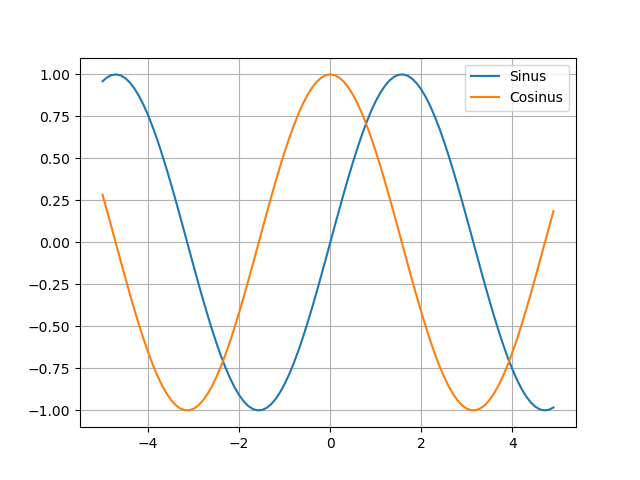
\includegraphics[width=\linewidth]{./gfx/plt-grid}
\end{tcolorbox}
%
\end{frame}

% =========================================================================== %

\begin{frame}[fragile]{Code Analysis}
%
\begin{itemize}
\item Multiple \texttt{plt.plot} lines
	\begin{itemize}
	\item Simply adds multiple lines
	\item Automatically picks new colour for each new line
	\end{itemize}
\item Optional argument \texttt{label}
	\begin{itemize}
	\item Text to put in the legend
	\item By default: empty string
	\item Not automatically displayed!
	\end{itemize}
\item \inPy{plt.leged()}
	\begin{itemize}
	\item Show a box with line colour and labels
	\end{itemize}
\item \inPy{plt.grid()}
	\begin{itemize}
	\item Show a grid
	\end{itemize}
\end{itemize}
%
\end{frame}

% =========================================================================== %

\begin{frame}[fragile]
%
\vspace{-5pt}
\begin{codebox}[Example: Headline and Axis Labels]
\begin{minted}[linenos, fontsize=\scriptsize]{python3}
import math
import matplotlib.pyplot as plt

h  = 6.62607015e-34     # Planck constant
T  = 300                # temperature in Kelvin
c  = 299792458          # speed of light
kB = 1.380649e-23       # Boltzmann constant

spectralDensity = lambda nu : ((2 * h * nu**3) / (c**2))  / \
                              (math.exp((h * nu) / (kB * T)) - 1)

X = [x for x in range(1, int(1e+14), int(1e+10))]
Y = [spectralDensity(x) for x in X]

plt.title ("Black Body Radiation")
plt.xlabel("Frequency of radiation in Hz")
plt.ylabel("Intensity in W/m²")

plt.plot(X, Y)
plt.show()
\end{minted}
\end{codebox}
%
%
\end{frame}

% =========================================================================== %

\begin{frame}[fragile]{Code Analysis}
%
\vspace{-10pt}
\begin{columns}[t]
\column{.5\linewidth}
\begin{itemize}
\item \texttt{plt.title} -- sets the plot title
\item \texttt{plt.xlabel} -- sets the label to the x axis
\item \texttt{plt.ylabel} -- guess what
\item Physics involved
	\begin{itemize}
	\item Heat makes bodies glow
	\item This computes the glow spectrum of a body at a given temperature
	\end{itemize}
\end{itemize}
%
\column{.5\linewidth}
\begin{tcolorbox}[title=Output: Headline and Axis Labels]
	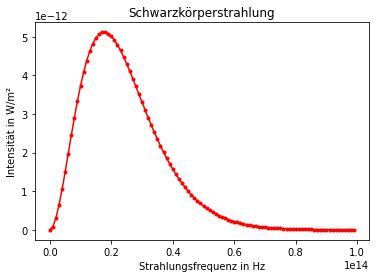
\includegraphics[width=\linewidth]{./gfx/plt-labels}
\end{tcolorbox}
\end{columns}
%
\end{frame}

% =========================================================================== %

\begin{frame}[fragile]
%
\begin{codebox}[Example: Linear and Logarithmic Plot]
\begin{minted}[linenos, fontsize=\scriptsize]{python3}
import matplotlib.pyplot as plt

W  = 500
X  = [x / 10 for x in range(-W, W)]
Y1 = [2 ** x for x in X]
Y2 = [x ** 7 for x in X]

plt.title("Linear Plot")
plt.plot(X, Y1, label="exponential")
plt.plot(X, Y2, label="power")
plt.legend()
plt.show()

plt.title("Logarithmic Plot")
plt.yscale("log")
plt.plot(X, Y1, label="exponential")
plt.plot(X, Y2, label="power")
plt.legend()
plt.show()
\end{minted}
\end{codebox}
%
\end{frame}

% =========================================================================== %

\begin{frame}[fragile]
%
\begin{tcbraster}[raster columns=2,
                  raster equal height,
                  nobeforeafter,
                  raster column skip=0.5cm]
\begin{tcolorbox}[title=Linear Plot]
	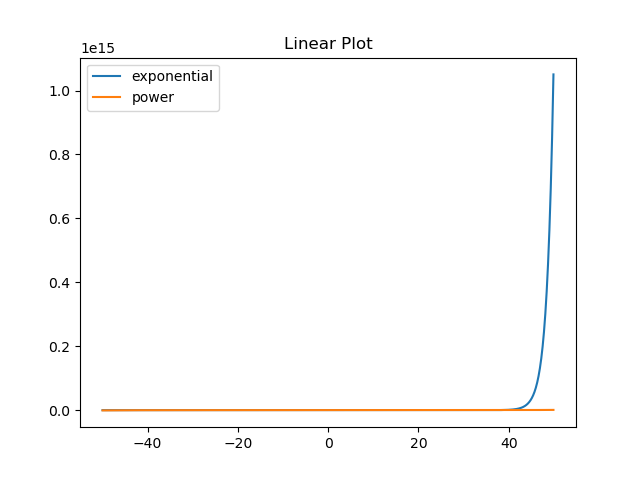
\includegraphics[width=\linewidth]{./gfx/plt-linear}
\end{tcolorbox}
%
\begin{tcolorbox}[title=Logarithmic Plot]
	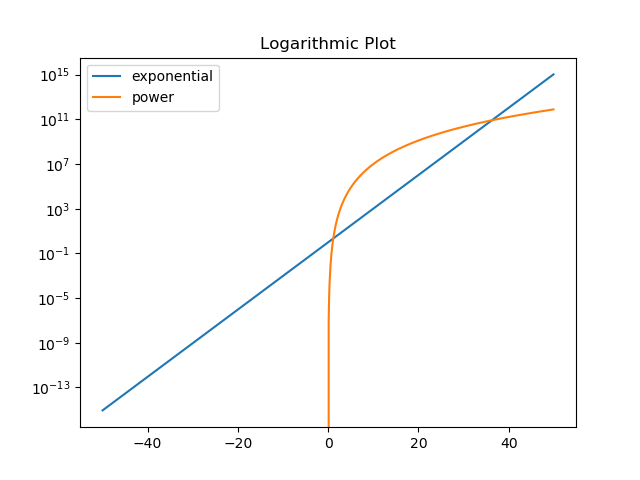
\includegraphics[width=\linewidth]{./gfx/plt-logarithmic}
\end{tcolorbox}
\end{tcbraster}
%
\end{frame}

% =========================================================================== %

\begin{frame}[fragile]{Logarithmic plots}
%
\begin{itemize}
\item Distort one or both axes to show highly dynamic processes
\item Equal distance -- constant factor
\item Doesn't work for negative values
\item Alternative: \inPy{"symlog"}
	\begin{itemize}
	\item \emph{symmetric logarithmic}
	\item Above [limit] and below -[limit]: logarithmic projection
	\item Between -[limit] and +[limit]: \emph{linear} projection
	\item limit: optional parameters \texttt{linthreshx} or \texttt{linthreshy}, respectively
	\end{itemize}
\end{itemize}
%
\end{frame}

% =========================================================================== %

\begin{frame}[fragile]
%
\begin{codebox}[Example: Symmetric Logarithmic Plots]
\begin{minted}[linenos, fontsize=\scriptsize]{python3}
import math
import matplotlib.pyplot as plt

W  = 500
X  = [x / 10 for x in range(-W, W)]
Y1 = [math.sin(x) for x in X]
Y2 = [x / 10      for x in X]

plt.xscale("symlog")
plt.plot(X, Y1)
plt.plot(X, Y2)
plt.grid()
plt.show()

plt.xscale("symlog", linthreshx=10)
plt.plot(X, Y1)
plt.plot(X, Y2)
plt.grid()
plt.show()
\end{minted}
\end{codebox}
%
\end{frame}

% =========================================================================== %

\begin{frame}[fragile]
%
\begin{tcbraster}[raster columns=2,
                  raster equal height,
                  nobeforeafter,
                  raster column skip=0.5cm]
\begin{tcolorbox}[title=symlog{,} default threshold]
	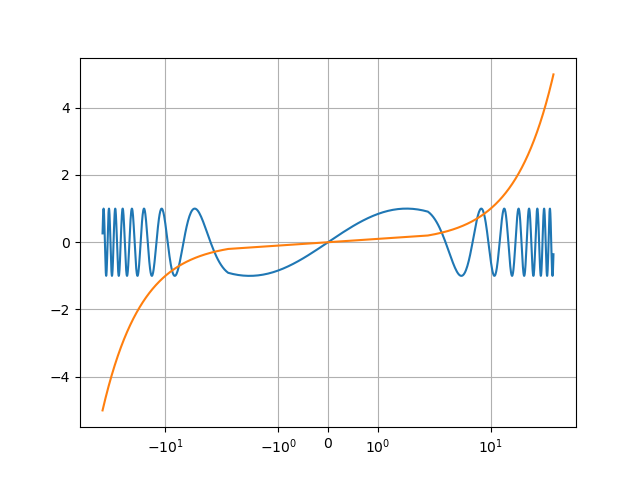
\includegraphics[width=\linewidth]{./gfx/plt-symlog}
\end{tcolorbox}
%
\begin{tcolorbox}[title=symlog{,} explicit threshold]
	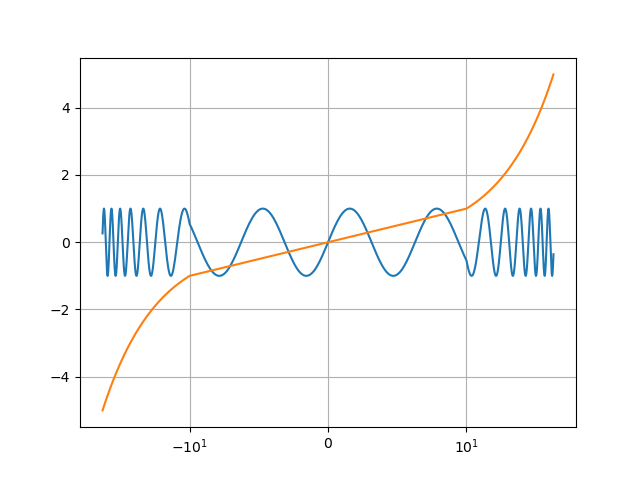
\includegraphics[width=\linewidth]{./gfx/plt-symlog-threshold}
\end{tcolorbox}
\end{tcbraster}
%
\end{frame}

% =========================================================================== %

\begin{frame}[fragile]
%
\begin{codebox}[Example: Manually Scaled Axes, width=.53\linewidth, nobeforeafter, equal height group = grpXmpSimplePlotScale]
\begin{minted}[linenos, fontsize=\scriptsize]{python3}
import math
import matplotlib.pyplot as plt

N = 100
X = [(x - N/2) / 10 for x in range(N)]
Y = [math.sin(x) for x in X]

plt.plot(X, Y)
plt.xlim(-6  , +6)
plt.ylim(-0.7, +3)
plt.grid()
plt.show()
\end{minted}
\end{codebox}
%
\begin{tcolorbox}[title=Output: Manually Scaled Axes, width=.45\linewidth, nobeforeafter, equal height group = grpXmpSimplePlotScale]
	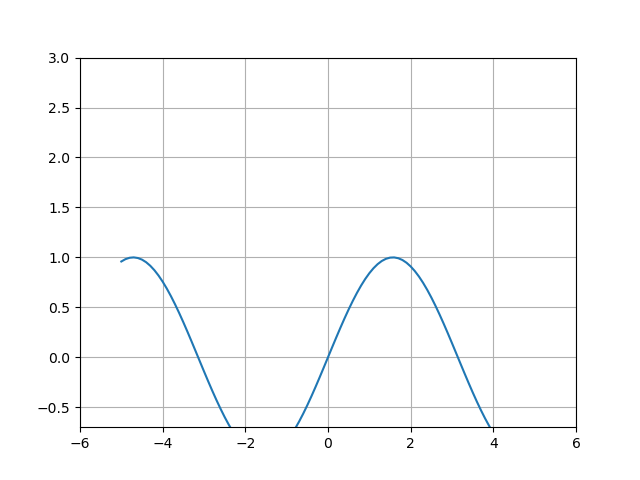
\includegraphics[width=\linewidth]{./gfx/plt-limits}
\end{tcolorbox}
%
\end{frame}

% =========================================================================== %

\begin{frame}[fragile]{Manually Formatting the Line}
%
\vspace{-10pt}
\begin{columns}[t]
\column{.5\linewidth}
\begin{itemize}
\item Optional parameters in the \texttt{plot} command
	\begin{itemize}
	\item String for most common options
	\item Keyword arguments for more details
	\end{itemize}
\item These control ...
	\begin{itemize}
	\item Line Color
	\item Line Style (solid, dashed, dash-dotted, ...)
	\item Marker (Type, edge- and face-color, ...)
	\item And a lot more
	\end{itemize}
\end{itemize}
%
Online Reference:
%
\column{.5\linewidth}
	\begin{tcolorbox}[title=Different Line Styles]
		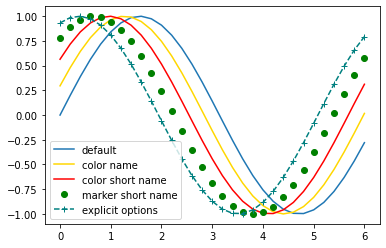
\includegraphics[width=\linewidth]{./gfx/plt-linestyles}
	\end{tcolorbox}
\end{columns}
%

\begin{itemize}
\item Line options: {\tiny \url{https://matplotlib.org/stable/api/_as_gen/matplotlib.lines.Line2D.html#matplotlib.lines.Line2D}}
\item Marker options: {\tiny \url{https://matplotlib.org/stable/api/markers_api.html#module-matplotlib.markers}}
\end{itemize}
%
\end{frame}

% =========================================================================== %

\begin{frame}[fragile]
%
\vspace{-5pt}
\begin{codebox}[Code: Different Line Styles]
\begin{minted}[linenos, fontsize=\scriptsize]{python3}
import math
import matplotlib.pyplot as plt

X = [x / 5 for x in range(31)]; Y = [math.sin(x) for x in X]
plt.plot(X, Y, label="default")

offset = .3; Y = [math.sin(x + offset) for x in X]
plt.plot(X, Y, "gold", label="color name")

offset += .3; Y = [math.sin(x + offset) for x in X]
plt.plot(X, Y, "r", label="color short name")

offset += .3; Y = [math.sin(x + offset) for x in X]
plt.plot(X, Y, "go", label="marker short name")

offset += .3; Y = [math.sin(x + offset) for x in X]
plt.plot(X, Y, color="#008080", linestyle="--", marker="+", label="explicit options")

plt.legend()
plt.show()
\end{minted}
\end{codebox}
%
\end{frame}

% =========================================================================== %

\begin{frame}
%
\vspace{-7pt}
\begin{tcolorbox}[title=Format Strings for \texttt{plt.plot()}]
\scriptsize
\begin{center}
	\begin{tabular}{cc|cc|cc}
		\multicolumn{6}{c}{\textbf{Marker Types}} \\
		Symbol     & Marker          & Symbol                    & Marker            & Symbol     & Marker                   \tabcrlf
		\texttt{,} & Pixel           & \texttt{.}                & small dot         & \texttt{o} & big dot                  \\
		\texttt{s} & Square          & \texttt{d}                & small diamond     & \texttt{D} & big diamond              \\
		\texttt{p} & Pentagon        & \texttt{h}                & Hexagon (upright) & \texttt{H} & Hexagon (recumbent)      \\
		\texttt{|} & Dash (vertical) & \texttt{+}                & Plus sign         & \texttt{x} & Cross                    \\
		\texttt{<} & Triangle (left) & \texttt{>}                & Triangle (right)  & \texttt{*} & Asterisk                 \\
		\texttt{v} & Triangle (down) & \texttt{\textasciicircum} & Triangle (up)     & \multicolumn{2}{c}{and some more ...} \\
	\end{tabular}
\end{center}

\begin{center}
	\begin{tabular}{cc|cc|cc|cc}
		\multicolumn{8}{c}{\textbf{Line Styles}} \\
		Symbol     & Line  & Symbol        & Line   & Symbol     & Line   & Symbol      & Line        \tabcrlf
		\texttt{-} & solid & \texttt{-{}-} & dashed & \texttt{:} & dotted & \texttt{-.} & dash-dotted \\
	\end{tabular}
\end{center}

\begin{center}
	\begin{tabular}{cc|cc|cc|cc}
		\multicolumn{8}{c}{\textbf{Colors}} \\
		Symbol     & Colour  & Symbol     & Colour  & Symbol     & Colour & Symbol     & Colour                \tabcrlf
		\texttt{b} & blue    & \texttt{c} & cyan    & \texttt{g} & green  & \texttt{k} & black (\enquote{key}) \\
		\texttt{m} & magenta & \texttt{r} & red     & \texttt{y} & yellow & \texttt{w} & white                 \\
	\end{tabular}
\end{center}
\end{tcolorbox}
%
\end{frame}

% =========================================================================== %

\begin{frame}[fragile]
%
\begin{codebox}[Example: Barplots, width=.58\linewidth, nobeforeafter, equal height group = grpXmpBarPlots]
\begin{minted}[linenos, fontsize=\scriptsize]{python3}
import matplotlib.pyplot as plt

X = ["Smoot", "Fnord", "R'lyeh"]
Y = [random.randint(0, 11) for x in X]
# this one goes up to eleven!

plt.bar(X, Y, color="#0040B0FF")
plt.ylim(0, 11)
plt.show()

plt.barh(X, Y, color="#0040B0FF")
plt.xlim(0, 11)
plt.show()
\end{minted}

\footnotesize
An optional string for styles as well as keyword arguments like \texttt{color} can be used, too.

\vspace{6pt}
Details:\\
{\tiny \url{https://matplotlib.org/3.1.1/api/_as_gen/matplotlib.pyplot.barh.html}}
\end{codebox}
%
\begin{tcolorbox}[title=Output: Barplots, width=.4\linewidth, nobeforeafter, equal height group = grpXmpBarPlots]
	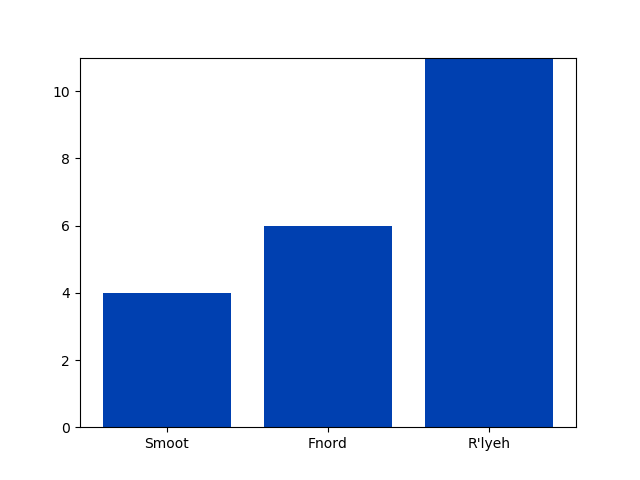
\includegraphics[width=\linewidth]{./gfx/plt-bars}
	
	\vspace{1pt}
	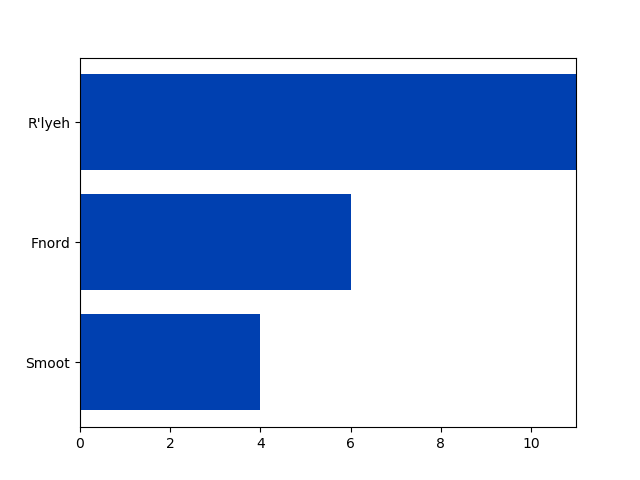
\includegraphics[width=\linewidth]{./gfx/plt-barh}
\end{tcolorbox}
%
\end{frame}

% =========================================================================== %

\begin{frame}[fragile]
%
\begin{codebox}[Example: Simple Pie Plot, width=.58\linewidth, nobeforeafter, equal height group = grpXmpPie1]
\begin{minted}[linenos, fontsize=\scriptsize]{python3}
import matplotlib.pyplot as plt

contributions = {
    "trial & error"               : 90,
    "searching the web"           : 50,
    "despair, fits of anger, etc" : 10,
    "writing small bits of code"  : 30,
    "brilliant ideas"             : 1
}

plt.pie( contributions.values() )
plt.show()
\end{minted}
\end{codebox}
%
\begin{tcolorbox}[title=Output: Simple Pie Plot, width=.4\linewidth, nobeforeafter, equal height group = grpXmpPie1]
	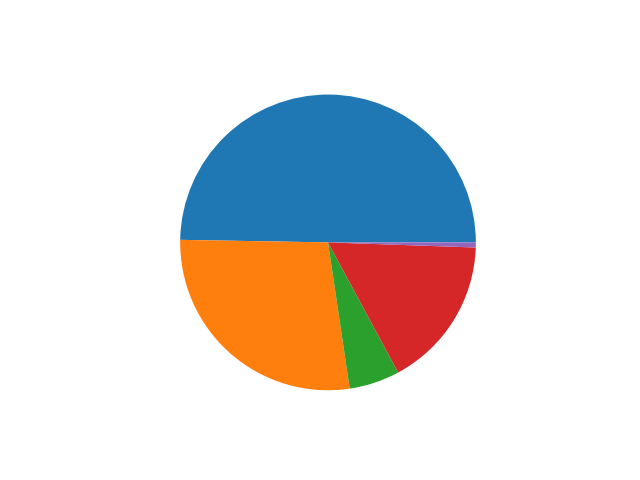
\includegraphics[width=\linewidth]{./gfx/plt-pie-simple}
\end{tcolorbox}
%
\begin{itemize}
\item Provide a container of numbers
\item Need not add up to 100
\item One slice per number, auto-coloured
\end{itemize}
%
\end{frame}

% =========================================================================== %

\begin{frame}[fragile]{Pie Plots: Optional Parameters}
%
\begin{columns}
\column{.85\linewidth}
\begin{center}
\begin{itemize}
\item[\texttt{labels}] Container of \inPy{str}ings to place next to slices
\item[\texttt{colors}] Container of \inPy{str}ings, names one colour for each slice
\item[\texttt{explode}] Container of \inPy{float}s, indicating how far to remove each slice from center, in units of pie radius
\item[\texttt{autopct}] \inPy{str}ing or function, specifies how to represent percentage
	\begin{itemize}
	\item C Style Format String: \texttt{\%.2f} -- floating point number with two decimal places
	\item Function \inPy{int} \thus \inPy{str}, takes value between 0 and 100 and computes what to write on the chart
	\item Details: \url{https://matplotlib.org/stable/api/_as_gen/matplotlib.pyplot.pie.html}
	\end{itemize}
\end{itemize}
\end{center}
\end{columns}
%
\end{frame}

% =========================================================================== %

\begin{frame}[fragile]
%
\vspace{-7pt}
\begin{codebox}[Example: Advanced Pie Plot]
\begin{minted}[linenos, fontsize=\scriptsize]{python3}
import matplotlib.pyplot as plt
contributions = {
    "trial & error"                 : 99, "searching the web"             : 50,
    "despair, fits of anger, etc"   : 10, "writing small bits\n of code"  : 30,
    "brilliant ideas"               : 1}

def percentToWords(x) :
    if        x <  5 : return "virtually nothing"
    elif  5 < x < 20 : return "a little"
    elif 20 < x < 50 : return "quite a bit"
    else             : return "the majority"

plt.title("Time Allocation in a coding project")
plt.xlabel("taken from experience")

plt.pie(
    contributions.values(), labels=contributions.keys(), autopct=percentToWords,
    colors=["#0000AAFF", "blue", "r", "green", "gold"], explode=(0, 0.1, 0, 0, .3)
)
plt.show()
\end{minted}
\end{codebox}
%
\end{frame}

% =========================================================================== %

\begin{frame}
%
\begin{tcolorbox}[title=Output: Advanced Pie Plot]
\begin{center}
	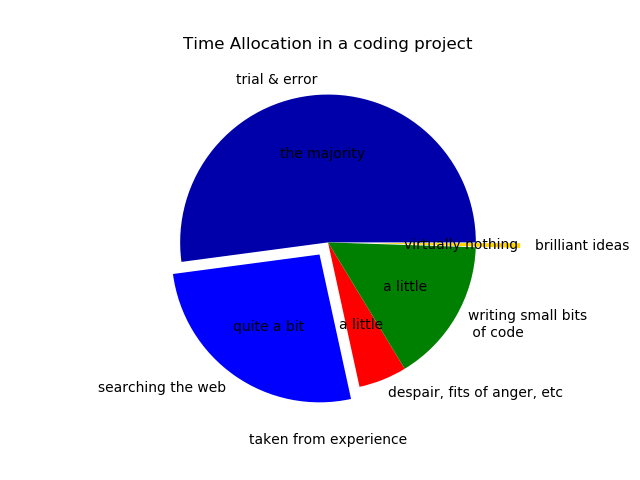
\includegraphics[width=.65\linewidth]{./gfx/plt-pie-args}
\end{center}
\end{tcolorbox}
%
\end{frame}

% =========================================================================== %

\begin{frame}[fragile]{Stackplots}
%
\begin{columns}
\column{.45\linewidth}
\begin{itemize}
\item Represent evolution of multiple populations that form a whole
\item Command \texttt{plt.stackplot}
\item First container: \enquote{time coordinate}
\item Subsequent containers: time evolution of populations
\item Optional parameters

	\begin{minipage}{.05\linewidth}
		\phantom{x}
	\end{minipage}
	\begin{minipage}{.90\linewidth}
		\begin{itemize}
		\item[labels] Container of \inPy{str}ings for legend
		\item[colors] Container of \inPy{str}ings with colour names
		\end{itemize}
	\end{minipage}
\end{itemize}
%
\column{.5\linewidth}
\begin{tcolorbox}[title=Stackplot]
	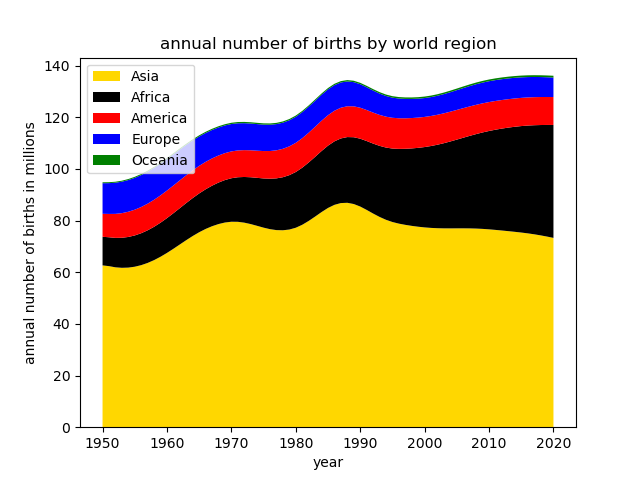
\includegraphics[width=\linewidth]{./gfx/plt-stackplot}
\end{tcolorbox}
\end{columns}
%
\end{frame}

% =========================================================================== %

\begin{frame}[fragile]
%
\begin{codebox}[Example: Stackplot ...]
\begin{minted}[linenos, fontsize=\scriptsize]{python3}
import csv
import matplotlib.pyplot as plt

years    = []
asia     = []
africa   = []
americas = []
europe   = []
oceania  = []
colors   = ["gold", "black", "red", "blue", "green"]

with open("annual-number-of-births-by-world-region.csv", "r") as handle :
    # Data from https://ourworldindata.org/world-population-growth
    # Contains data like:
    # Year,Asia,Africa,America,Europe,Oceania
    # 1950,11071.722,8896.969,62638.002,11837.577,360.997
    # 1951,11178.006,9031.823,62344.074,11917.33,366.362
    # ...
      
    reader = csv.reader(handle)

\end{minted}
\end{codebox}
%
\end{frame}

% =========================================================================== %

\begin{frame}[fragile]
%
\begin{codebox}[... continued]
\begin{minted}[linenos, fontsize=\scriptsize, firstnumber=last]{python3}
    labels = next(reader)[1:]    # read first line;
                                 # take column heads except for first ("Year")

    for line in reader :         # read the rest of the file
        years   .append(float(line[0])       )
        africa  .append(float(line[1]) / 1000)  # line[i] / 1000: Data are given
        americas.append(float(line[2]) / 1000)  # in thousands; we want our plot
        asia    .append(float(line[3]) / 1000)  # to be in millions.
        europe  .append(float(line[4]) / 1000)
        oceania .append(float(line[5]) / 1000)

plt.title ("annual number of births by world region")
plt.xlabel("year")
plt.ylabel("annual number of births in millions")
plt.legend(loc="upper left")

plt.stackplot(years,
              asia, africa, americas, europe, oceania,
              labels=labels, colors=colors)
plt.show()
\end{minted}
\end{codebox}
%
\end{frame}

% =========================================================================== %

\begin{frame}[fragile]{Scatterplots}
%
\vspace{-15pt}
\begin{columns}[t]
\column{.49\linewidth}
\begin{itemize}
\item Up to four independent variables at once
\item x, y, size, colour
\item colour: numbers or colour names
\item Optional parameters

	\begin{minipage}{.10\linewidth}
		\phantom{x}
	\end{minipage}
	\begin{minipage}{.85\linewidth}
		\begin{itemize}
		\item[marker] String or Marker object
		\item[cmap] \enquote{Colour Map}, either a string with a map name or a complex object. Default: \inPy{"viridis"} (purple, blue, green, yellow)
		\end{itemize}
	\end{minipage}

\item Details:\\
{\scriptsize\url{https://matplotlib.org/stable/api/_as_gen/matplotlib.pyplot.scatter.html}}
\end{itemize}
%
\column{.45\linewidth}
\vspace{-10pt}
\begin{tcolorbox}[title=Germany as Scatterplot]
\begin{center}
	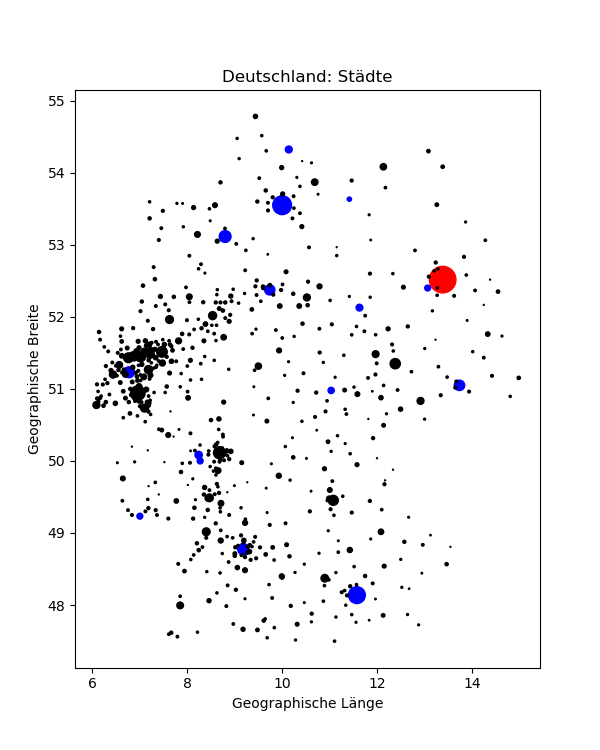
\includegraphics[width=.8\linewidth]{./gfx/plt-de}
\end{center}
\end{tcolorbox}
\end{columns}
%
\end{frame}

% =========================================================================== %

\begin{frame}[fragile]
%
\begin{codebox}[Code: Germany as Scatterplot ...]
\begin{minted}[linenos, fontsize=\scriptsize]{python3}
import csv
import matplotlib.pyplot as plt

colors = {"primary" : "red", "admin" : "blue", "minor" : "black"}
         # federal capital , state capital   , other city

lat = []; lng = []     # geographic latitude and longitude
pop = []; col = []     # population and dot colour

sizer = lambda x : 0.5 if x < 10000 else x / 10000   # compute size of dots, minimum 0.5

with open("cities-locations-populations-Germany.csv", "r") as handle :
    # Data from https://simplemaps.com/data/de-cities
    # Contains lines like:
    # city,lat,lng,country,iso2,admin_name,capital,population,population_proper
    # Berlin,52.5167,13.3833,Germany,DE,Berlin,primary,3644826,3644826
    # Hamburg,53.5500,10.0000,Germany,DE,Hamburg,admin,1841179,1841179
    # ...
    
    reader = csv.reader(handle)
\end{minted}
\end{codebox}
%
\end{frame}

% =========================================================================== %

\begin{frame}[fragile]
%
\begin{codebox}[... continued]
\begin{minted}[linenos, fontsize=\scriptsize, firstnumber=last]{python3}
    next(reader)
    
    for line in reader :
            lat.append(float(line[1]))
            lng.append(float(line[2]))
            pop.append( sizer(float(line[7]))  )
            col.append( colors[line[6]] )

plt.figure(figsize=(6,7.5))
plt.title("Deutschland: Städte")
plt.xlabel("Geographische Länge")
plt.ylabel("Geographische Breite")
plt.scatter(lng, lat, pop, col)
plt.show()
\end{minted}
\end{codebox}
%
\end{frame}

% =========================================================================== %

\begin{frame}[fragile]{Quiver Plots: Vector Fields}
%
\vspace{-15pt}
\begin{columns}[t]
\column{.49\linewidth}
\begin{itemize}
\item \enquote{Map of arrows}
\item Input: 4 lists or generic containers
	\begin{itemize}
	\item \texttt{X}, \texttt{Y}, \texttt{arrow\_X}, \texttt{arrow\_Y}
	\item \texttt{X}, \texttt{Y} can be ommitted
	\item \texttt{arrow\_X}, \texttt{arrow\_Y} then need to be lists of lists
	\item One list per line
	\end{itemize}

\item Details:\\
{\scriptsize\url{https://matplotlib.org/3.1.1/api/_as_gen/matplotlib.pyplot.quiver.html}}
\end{itemize}
%
\column{.45\linewidth}
\vspace{-10pt}
\begin{tcolorbox}[title=Quiver Plot]
	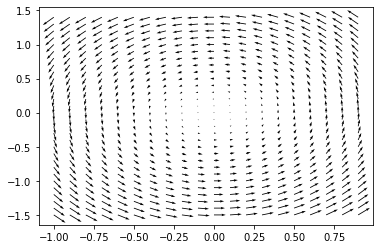
\includegraphics[width=\linewidth]{./gfx/plt-vortex}
\end{tcolorbox}
\end{columns}
%
\end{frame}

% =========================================================================== %

\begin{frame}[fragile]
%
\begin{codebox}[Code: Quiver Plot]
\begin{minted}[linenos, fontsize=\scriptsize]{python3}
import matplotlib.pyplot as plt

width = 10; height = 15

xPoints = [x / 10 for x in range(- width, + width)]
yPoints = [y / 10 for y in range(-height, +height)]

Nx = len(xPoints); Ny = len(yPoints)

X = []; Y = []

for i in range(Ny) : X.extend(  xPoints          )    # alt. spelling of X += xPoints
for i in range(Ny) : Y.append( [yPoints[i]] * Nx )

# vector field: v = (y, -x)
U = Y.copy(); V = X.copy()
for i, v in enumerate(V) : V[i] = -v

plt.quiver(X, Y, U, V)
plt.show()
\end{minted}
\end{codebox}
%
\end{frame}

% =========================================================================== %

\begin{frame}{And so much more...}
%
\begin{itemize}
\item Histograms
\item Boxplots
\item Confidence Intervals and Error Bars
\item 3D Plots and Contour Maps (actually presented next lecture)
\item See \url{https://matplotlib.org/stable/plot_types/index.html}
\end{itemize}
%
\end{frame}